\chapter{Introduction}
This document describe a SPI Slave core designed for the Xilinx EDK. \cite{bib_xilinx_edk}

\section{Features}
\begin{itemize}
\item OPB-Clock and SPI-Clock are complete independent
\item SPI can run faster than OPB if guaranteed that no TX-FIFO Underrunn or RX-FIFO Overrunn occure.
\item variable transfer length 2..32
\end{itemize}




\section{Limitations}
\begin{itemize}
\item designed only for Xilinx Spartan-3/Virtex-4 at the moment
\item only Slave Operation
\end{itemize}

\chapter{Core configuration}
\begin{table} [h]
	\centering
		\begin{tabular} {|l|l|c|c|} \hline
			Description							& Parameter Name & Allowable Values	& Default Value	\\ \hline
			\multicolumn{4} {|c|} {System Parameter} \\ \hline			
 		  Base address for OPB SPI& C\_BASEADDR		 & 0x00							& 0x00000000		\\ \hline
 		  High address for OPB SPI& C\_HIGHADDR		 & BASEADDR+0x3F		& BASEADDR+0x3f \\ \hline
		  OPB address bus width		& C\_OPB\_AWIDTH & 32								& 32						\\ \hline
 		  OPB data bus width  		& C\_OPB\_DWIDTH & 32								& 32						\\ \hline
 		  Target FPGA Family  	  & C\_FAMILY			 & spartan3,virtex4 & virtex4		  	\\ \hline
		  \multicolumn{4} {|c|} {User Parameter} \\ \hline
			Shift register width		& C\_SR\_WIDTH	 & 8-32							& 8							\\ \hline	
			Shift MSB First				  & C\_MSB\_FIRST  & true, false			& true			   	\\ \hline
			SPI Clock Polarity		  & C\_CPOL				 & 0,1							&	0							\\ \hline
			SPI Clock Phase				  & C\_CPHA				 & 0,1							&	0							\\ \hline
  		FIFO Size Width(TX/RX)\footnotemark[1]	& C\_FIFO\_DEPTH & 4-7							&	4  						\\ \hline
			DMA\_EN			   				  & C\_DMA\_EN		 & true, false			&	false					\\ \hline	
		\end{tabular}
	\caption{Generics}
	\label{tab:Generics}
\end{table}

\footnotetext[1]{FIFO depth is $2^{Value}$ =(16,32,64,128)}



\chapter{IO-Ports}
\begin{table} [h]
	\centering
		\begin{tabular}{|l|l|l|l|} \hline
		\textbf{Port}		& \textbf{width}	& \textbf{direction}	& \textbf{Description} \\ \hline
		SPI\_SCLK				& 1		& input			& Serial clock input	\\
		SPI\_MOSI				& 1		& input			& Master Out Slave in \\
		SPI\_MISO				& 1 	& output		& Master in Slave out	\\
		SPI\_SS					& 1		& input			& Slave select				\\ \hline
		opb\_irq				& 1		& output		& IRQ Output					\\ \hline
		\end{tabular}
	\caption{external ports}
	\label{tab:externalPorts}
\end{table}

\chapter{Registers}
\section{Adressmap}
\begin{table} [!h]
	\centering
		\begin{tabular}{|l|c|c|l|} \hline
		\textbf{Name}		& \textbf{Adress}	& \textbf{Acess}	& \textbf{Description} 				\\ \hline
		SPI\_CR					& 0x00						& R/W							& SPI Control Register				\\ \hline
		SPI\_SR					& 0x04						& R/W							& SPI  Status Register				\\ \hline
		SPI\_TD					& 0x08						& W								& SPI Transmit Data  Register \\ \hline
		SPI\_RD					& 0x0C						& R								& SPI Receive Data  Register 	\\ \hline		
		TX\_THRESH	  	& 0x10						& R/W							& TX-Threshold Prog Full/Emty	\\ \hline
		RX\_THRESH		  & 0x14						& R/W							& RX-Threshold Prog Full/Emty \\ \hline		
		TX\_DMA\_CTL		& 0x18						& R/W							& TX DMA Control							\\ \hline
		TX\_DMA\_ADDR		& 0x1C						& R/W							& TX DMA Base Adress Offset		\\ \hline	
		TX\_DMA\_NUM		& 0x20						& R/W							& TX DMA Number of Transfers	\\ \hline	
		RX\_DMA\_CTL		& 0x24						& R/W							& RX DMA Control							\\ \hline
		RX\_DMA\_ADDR		& 0x28						& R/W							& RX DMA Base Adress Offset		\\ \hline	
		RX\_DMA\_NUM		& 0x2C						& R/W							& RX DMA Number of Transfers	\\ \hline	
							
		DGIE	  				& 0x40						& R/W							& Device global IRQ Enable Register	\\ \hline	
		IPISR	   				& 0x44						& R/W							& IRQ Status Register	  			\\ \hline	
		IPIER	   				& 0x48						& R/W							& IRQ Enable Register	  			\\ \hline			
		\end{tabular}
	\caption{Address-Map}
	\label{tab:registers}
\end{table}

\section{SPI\_CR}
\begin{table} [!h]
	\centering
		\begin{tabular} {|l|c|c|c|l|} \hline
		\textbf{Bit}		& \textbf{Name}	& \textbf{Acess} & \textbf{Reset Value}	& \textbf{Description} 				\\ \hline
	  31							& DGE						& R/W						 & 0										& Device Global Enable				\\
	  								&								&								 &											& 0: Disable 									\\
	  								&								&								 &											& 1: Enable 	  							\\ \hline		
	  30							& TX\_EN				& R/W						 & 0										& Transmit Enable	  					\\
	  								&								&								 &											& 0: Disable 									\\
	  								&								&								 &											& 1: Enable 	  							\\ \hline	
	  29							& RX\_EN				& R/W						 & 0										& Receive Enable	  					\\
	  								&								&								 &											& 0: Disable 									\\
	  								&								&								 &											& 1: Enable 	  							\\ \hline		 	
	  29							& RESET					& R/W						 & 0										& Reset Device(self cleared)	\\
	  								&								&								 &											& 0: Normal Operation					\\
	  								&								&								 &											& 1: Reset SPI-Core(SR/FIFO)  \\ \hline			  		29..0						& 	\multicolumn{4} {c|} {reserved} \\ \hline																														\end{tabular}
	\caption{SPI\_CR Register}
	\label{tab:SPI_CR}
\end{table}


\section{SPI\_SR}
\begin{table} [!h]
	\centering
		\begin{tabular} {|l|l|c|c|l|} \hline
		\textbf{Bit}		& \textbf{Name}	& \textbf{Acess} & \textbf{Reset Value}	& \textbf{Description} 				\\ \hline
	  31							& TX Prog Full	& R							 & 0										& Prog Full Flag 	  					\\
	  								&								&								 &											& 1: FIFO Prog Full 					\\ \hline
	  30							& TX Full				& R							 & 0										& Full Flag 	  							\\
	  								&								&								 &											& 1: FIFO Full 								\\ \hline
	  29							& TX Overflow		& R							 & 0										& Overflow Flag 							\\
	  								&								&								 &											& 1: FIFO Overflow						\\ 
	  								&								&								 &											& (Cleared only at Reset)			\\ \hline	  		
	  28							& TX Prog Empty & R							 & 0										& Prog Empty Flag 	  				\\
	  								&								&								 &											& 1: FIFO Prog Empty 		 			\\ \hline
	  27							& TX Empty			& R							 & 0										& Full Flag 	  							\\
	  								&								&								 &											& 1: FIFO Empty								\\ \hline
	  26							& TX Underflow	& R							 & 0										& Underflow Flag 							\\
	  								&								&								 &											& 1: FIFO Underflow						\\ 
	  								&								&								 &											& (Cleared only at Reset)			\\ \hline	 
	  25							& RX Prog Full	& R							 & 0										& Prog Full Flag 	  					\\
	  								&								&								 &											& 1: FIFO Prog Full 					\\ \hline
	  24							& RX Full				& R							 & 0										& Full Flag 	  							\\
	  								&								&								 &											& 1: FIFO Full 								\\ \hline
	  23							& RX Overflow		& R							 & 0										& Overflow Flag 							\\
	  								&								&								 &											& 1: FIFO Overflow						\\ 
	  								&								&								 &											& (Cleared only at Reset)			\\ \hline	  		
	  22							& RX Prog Empty & R							 & 0										& Prog Empty Flag 	  				\\
	  								&								&								 &											& 1: FIFO Prog Empty 		 			\\ \hline
	  21							& RX Empty			& R							 & 0										& Full Flag 	  							\\
	  								&								&								 &											& 1: FIFO Empty								\\ \hline
	  20							& RX Underflow	& R							 & 0										& Underflow Flag 							\\
	  								&								&								 &											& 1: FIFO Underflow						\\ 
	  								&								&								 &											& (Cleared only at Reset)			\\ \hline	
	  19							& Chip Select  	& R							 & 0										& Chip Select Flag						\\
	  								&								&								 &											& 0: CS\_N Low								\\ 
	  								&								&								 &											& 1: CS\_N High								\\ \hline
	  18							& TX DMA Done 	& R							 & 0										& Transmit DMA done						\\
	  								&								&								 &											& 0: TX DMA in progress				\\ 
	  								&								&								 &											& 1: TX DMA all Transfers done\\ \hline	  		  17							& RX DMA Done 	& R							 & 0										& Receive DMA done						\\
	  								&								&								 &											& 0: RX DMA in progress				\\ 
	  								&								&								 &											& 1: RX DMA all Transfers done\\ \hline	  	
 		16..0						& 	\multicolumn{4} {c|} {reserved} \\ \hline																														\end{tabular}
	\caption{SPI\_SR Register}
	\label{tab:SPI_SR}
\end{table}

\newpage
\section{TX\_THRESH}
\begin{table}[!h]
	\centering
		\begin{tabular} {|l|l|c|c|l|} \hline
		\textbf{Bit}		& \textbf{Name}	& \textbf{Acess} & \textbf{Reset}				& \textbf{Description} 				\\ 
										&								&								 & \textbf{Value}				&															\\ \hline		
	  31..16					& TX\_THRESH\_PROG\_FULL 	& R/W	 & 0										& Transmit Prog Full Threshold\\
	  								&								&								 &											& [1..$2^{C\_FIFO\_DEPTH}-2$]	\\ \hline
	  15..0						& TX\_THRESH\_PROG\_EMPTY	& R/W	 & 0										& Transmit Prog Empty	Threshold\\
	  								&								&								 &											& [1..$2^{C\_FIFO\_DEPTH}-2$]	\\ \hline
	\end{tabular}
	\caption{TX\_THRESH Register}
	\label{tab:TX_THRESH}
\end{table}


\section{RX\_THRESH}
\begin{table}[!h]
	\centering
		\begin{tabular} {|l|l|c|c|l|} \hline
		\textbf{Bit}		& \textbf{Name}	& \textbf{Acess} & \textbf{Reset}				& \textbf{Description} 				\\
										&								&								 & \textbf{Value}				&															\\ \hline
	  31..16					& RX\_THRESH\_PROG\_FULL 	& R/W	 & 0										& Receive Prog Full Threshold	\\
	  								&								&								 &											& [1..$2^{C\_FIFO\_DEPTH}-2$] \\ \hline
	  15..0						& RX\_THRESH\_PROG\_EMPTY	& R/W	 & 0										& Receive Prog Empty Threshold\\
	  								&								&								 &											& [1..$2^{C\_FIFO\_DEPTH}-2$] \\ \hline					\end{tabular}
	\caption{RX\_THRESH Register}
	\label{tab:RX_THRESH}
\end{table}


\section{DGIE}
\begin{table} [!h]
	\centering
		\begin{tabular} {|l|c|c|c|l|} \hline
		\textbf{Bit}		& \textbf{Name}	& \textbf{Acess} & \textbf{Reset Value}	& \textbf{Description} 				\\ \hline
	  31							& DGIE					& R/W						 & 0										& Global IRQ Ebable  					\\
	  								&								&								 &											& 0: Disable 									\\
	  								&								&								 &											& 1: Enable 	  							\\ \hline		
 		29..0						& 	\multicolumn{4} {c|} {reserved} \\ \hline																														\end{tabular}
	\caption{DGIE Register}
	\label{tab:dgie}
\end{table}

\newpage
\section{IPISR}
\begin{table} [!h]
	\centering
		\begin{tabular} {|l|l|c|c|l|} \hline
		\textbf{Bit}		& \textbf{Name}	& \textbf{Acess} & \textbf{Reset Value}	& \textbf{Description} 				\\ \hline
	  31							& TX\_Prog\_Empty & R/ToW\footnotemark[1]	 & 0										& IRQ Prog Empty Flag 	  		\\ \hline
	  29							& TX\_Empty			& R/ToW					 & 0										& IRQ Full Flag 							\\ \hline
	  28							& RX\_Prog\_Full& R/ToW					 & 0										& IRQ Prog Full Flag 	  			\\ \hline
	  27							& RX\_Full			& R/ToW 				 & 0										& IRQ Full Flag  							\\ \hline
	  26							& SS\_FALL			& R/ToW					 & 0										& IRQ SS FALL Flag						\\ \hline
	  25							& SS\_RISE			& R/ToW					 & 0										& IRQ SS RISE Flag						\\ \hline
 		24..0						& 	\multicolumn{4} {c|} {reserved} \\ \hline																														\end{tabular}
	\caption{IPISR Register}
	\label{tab:IPISR}
\end{table}

\footnotetext[1]{Read and ToggleOnWrite (writing 1 clears the bit)}

\section{IPISE}
\begin{table} [!h]
	\centering
		\begin{tabular} {|l|l|c|c|l|} \hline
		\textbf{Bit}		& \textbf{Name}			& \textbf{Acess} & \textbf{Reset Value}	& \textbf{Description} 				\\ \hline
	  31							& TX\_Prog\_Empty 	& R/W						 & 0										  & IRQ Prog Empty Enable 		\\ \hline
	  29							& TX\_Empty					& R/W						 & 0										& IRQ Full Enable							\\ \hline
	  28							& RX\_Prog\_Full		& R/W						 & 0										& IRQ Prog Full Enable  			\\ \hline
	  27							& RX\_Full					& R/W						 & 0										& IRQ Full Enable							\\ \hline
	  26							& SS\_FALL	  			& R/W						 & 0										& IRQ SS FALL Enable 					\\ \hline
	  25							& SS\_RISE					& R/W						 & 0										& IRQ SS RISE Enable				  \\ \hline
	  24							& TX\_DMA\_DONE			& R/W						 & 0										& IRQ TX Transfer done	Enable\\ \hline
	  23							& TX\_DMA\_DONE			& R/W						 & 0										& IRQ RX Transfer done	Enable\\ \hline	   	 22..0					 & 	\multicolumn{4} {c|} {reserved} \\ \hline																														\end{tabular}
	\caption{IPISE Register}
	\label{tab:IPISE}
\end{table}

1: IRQ enabled

\chapter{System Integration}
To integrate this IP-Core in your System, unzip the opb\_spi\_slave.zip to your project-directory. Then Rescan the user repository with \textit{Project $\rightarrow$ Rescan User Repositories}. This will take some seconds. After this you find the core in the \textit{IP Catalog $\rightarrow$ Project Repository}.

\section{MPD-File}
\begin{verbatim}
BEGIN opb_spi_slave
 PARAMETER INSTANCE = opb_spi_slave_0
 PARAMETER HW_VER = 1.00.a
 PARAMETER C_BASEADDR = 0x7d600000
 PARAMETER C_HIGHADDR = 0x7d60ffff
 BUS_INTERFACE MSOPB = mb_opb
 PORT sclk = opb_spi_slave_0_sclk
 PORT ss_n = opb_spi_slave_0_ss_n
 PORT mosi = opb_spi_slave_0_mosi
 PORT miso = opb_spi_slave_0_miso
 PORT opb_irq = opb_spi_slave_0_opb_irq
END
\end{verbatim}

\section{UCF-File}
\begin{verbatim}
# assign I/O Pins 
NET opb_spi_slave_0_sclk_pin LOC= AA24; # must CC capable IO in virtex-4
NET opb_spi_slave_0_ss_n_pin LOC= V20;
NET opb_spi_slave_0_mosi_pin LOC= AC25;
NET opb_spi_slave_0_miso_pin LOC= AC24;
NET opb_spi_slave_0_miso_pin SLEW = FAST;

#### Module OPB_SPI_Slave constraints
Net opb_spi_slave_0_sclk_pin TNM_NET = spi_clk;
TIMESPEC TS_spi_clk = PERIOD spi_clk 40 ns;

NET "opb_spi_slave_0_mosi_pin" TNM = "spi_in";
#NET "opb_spi_slave_0_cs_n_pin" TNM = "spi_in";
TIMEGRP "spi_in" OFFSET = IN 5 ns VALID 10 ns BEFORE "opb_spi_slave_0_sclk_pin" HIGH ;

NET "opb_spi_slave_0_miso_pin" TNM = "spi_out";
TIMEGRP "spi_out" OFFSET = OUT 14 ns AFTER "opb_spi_slave_0_sclk_pin" LOW ;
\end{verbatim}

\section{Register Header}

\verbatiminput{opb_spi_slave.h}


\chapter{Operations}

\chapter{Architecture}

\begin{figure}[h]
	\centering
		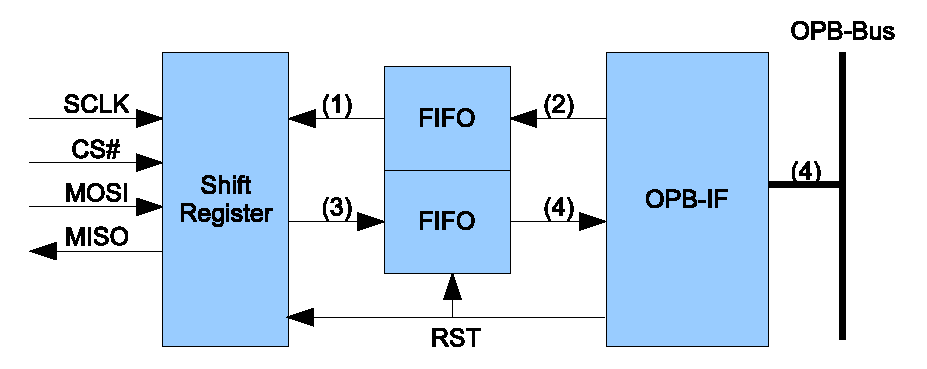
\includegraphics[width=1.00\textwidth]{Grafik/block_diagramm}
	\caption{Blockdiagramm}
	\label{fig:blockdiagramm}
\end{figure}

\section{Serial Shift Register}
\begin{table}[!h]
	\centering
		\begin{tabular} {|l|c|l|} \hline \rowcolor{yellow1}
		\textbf{Signal}		& \textbf{Direction}& \textbf{Description}	\\ \hline
		\multicolumn{3} {c|} {Generics} \\ \hline		
		C\_SR\_WIDTH	 									& -									& Shift register width  \\ \hline	
		C\_MSB\_FIRST  									& -									& Transfer MSB First		\\ \hline		
		\multicolumn{3} {c|} {Global} \\ \hline			
		rst					 										& input							& Async-Reset						\\ \hline		
		\multicolumn{3} {c|} {External Interface} \\ \hline		
		sclk														& input							& Serial clock input		\\ \hline
		cs\_n														& input							& Chip Select						\\ \hline
		mosi														& input							& Master Out Slave in 	\\ \hline
		miso\_o													&	output						& Master in Slave out		\\ \hline
		miso\_i													& input							& not used							\\ \hline
		miso\_t													& output						& MISO Tristate		  		\\ \hline	
		\multicolumn{3} {c|} {TX-FIFO (1)} \\ \hline	
		sr\_tx\_clk											& output						& FIFO-TX CLK					\\ \hline
		sr\_tx\_en  										& output						& FIFO-TX enable			\\ \hline	
		sr\_tx\_data[C\_SR\_WIDTH:0]		& input							& FIFO-TX Data				\\ \hline
		\multicolumn{3} {c|} {RX-FIFO (3)} \\ \hline	
		sr\_rx\_clk											& output						& FIFO-RX CLK					\\ \hline
		sr\_rx\_en  										& output						& FIFO-RX enable			\\ \hline	
		sr\_rx\_data[C\_SR\_WIDTH:0]	  & output						& FIFO-RX Data				\\ \hline
		\end{tabular}
	\caption{Serial-Register}
	\label{tab:SerialRegister}
\end{table}
\clearpage

\section{FIFO}
\begin{table}[!h]
	\centering
		\begin{tabular} {|l|c|l|} \hline \rowcolor{yellow1}
		\textbf{Signal}							& \textbf{Direction}& \textbf{Description}	\\ \hline
		\multicolumn{3} { c|} {Generics} \\ \hline		
		C\_FIFO\_WIDTH 							& -									& Shift register width  \\ \hline	
		C\_FIFO\_SIZE								& -									& FIFO Size Width				\\ \hline
		C\_SYNC\_TO									& -									& FIFO Sync Flags to Clock \\ \hline
		\multicolumn{3} { c|} {Global} \\ \hline	
		rst					 								& input							& Async-Reset						\\ \hline	
		\multicolumn{3} { c|} {Write-Port (2,3)} 				\\ \hline	
		wr\_clk											& input							& FIFO Write CLK				\\ \hline
		wr\_en  										& input							& FIFO Write enable			\\ \hline	
		din[C\_FIFO\_WIDTH:0]				& input							& FIFO Write data				\\ \hline
		\multicolumn{3} { c|} {READ-Port (1,4)} 				\\ \hline	
		rd\_clk											& input							& FIFO Read CLK					\\ \hline
		rd\_en  										& input							& FIFO Read enable			\\ \hline	
		dout[C\_FIFO\_WIDTH:0]			& output						& FIFO Read data				\\ \hline
		\multicolumn{3} { c|} {Flags (4)}								\\ \hline			
		empty												& output						& FIFO Emtpy						\\ \hline
		full												& output						& FIFO Full							\\ \hline
		overflow										& output						& FIFO Overflow 				\\ \hline
		underflow										& output						& FIFO Underflow				\\ \hline
		prog\_full\_thresh[C\_FIFO\_WIDTH:0]	& output	& FIFO Programmable Full Threshold \\ \hline
		prog\_empty\_thresh[C\_FIFO\_WIDTH:0]	& output	& FIFO Programmable Empty	Threshold\\ \hline
		prog\_full									& output						& FIFO Programmable Full  \\ \hline
		prog\_empty									& output						& FIFO Programmable Empty	\\ \hline
		\end{tabular}
	\caption{TX-FIFO}
	\label{tab:tx-fifo}
\end{table}
 
\newpage   
\section{OPB\_IF}
\begin{table}[!h]
	\centering
		\begin{tabular} {|l|c|l|} \hline \rowcolor{yellow1}
		\textbf{Signal}							& \textbf{Direction}& \textbf{Description}	\\ \hline
		\multicolumn{3} { c|} {Generics} \\ \hline		
 		C\_BASEADDR		 						& -							 		  & Base address for OPB SPI		\\ \hline
    C\_HIGHADDR									& - 								& High address for OPB SPI	  \\ \hline
		C\_OPB\_AWIDTH 							& - 								& OPB address bus width			  \\ \hline
 		C\_OPB\_DWIDTH 							& - 								& OPB data bus width					\\ \hline
 		C\_FAMILY			 							& - 								& Target FPGA Family	  			\\ \hline
		C\_SR\_WIDTH	 							& -									& Shift register width  			\\ \hline	 		  
		C\_FIFO\_WIDTH 							& -									& Shift register width  			\\ \hline	
		C\_FIFO\_SIZE								& -									& FIFO Size Width							\\ \hline
		C\_NUM\_FLG									& - 								& Number of FIFO Status flags	\\ \hline
		C\_NUM\_INT									& - 								& Number of IRQ Sources				\\ \hline
		\multicolumn{3} { c|} {OPB-Bus} \\ \hline	
		OPB\_rst			 							& input							& Async-Reset									\\ \hline	
    OPB\_ABus[C\_OPB\_AWIDTH-1:0]	& input      			& Adress-Bus									\\ \hline	
    OPB\_BE[C\_OPB\_DWIDTH/8-1:0]	& input				    & Bytes Enables								\\ \hline 
    OPB\_Clk 										& input							& Clock												\\ \hline							     
    OPB\_DBus[C\_OPB\_DWIDTH-1:0]	& input						& Data-Bus to slave						\\ \hline
    OPB\_RNW      							& input							& Read/Write									\\ \hline
    OPB\_Rst      							& input							& Reset												\\ \hline
    OPB\_select  								& input							& Select 											\\ \hline											
    OPB\_seqAddr 								& input							& Sequential Adress Enable		\\ \hline 
    Sln\_DBus     							& output						& Data-Bus to Master					\\ \hline
    Sln\_errAck   							& output						& Error Acknowledge   				\\ \hline		
    Sln\_retry    							& output						& Retry 											\\ \hline		
    Sln\_toutSup  							& output						& Timeout Suppression					\\ \hline		
    Sln\_xferAck 								& output						& transfer Acknowledge				\\ \hline	
		\multicolumn{3} { c|} {FIFO-PORT (2)} 								\\ \hline
    opb\_tx\_en    							& output						& FIFO-TX Write Enable				\\ \hline
    opb\_tx\_data[C\_SR\_WIDTH:0] 	& output				& FIFO-TX Write Data					\\ \hline
		tx\_thresh[(2*C\_FIFO\_SIZE)-1:0]	& output			& FIFO-TX Prog Thresholds			\\ \hline   
		\multicolumn{3} { c|} {FIFO-PORT (4)} 								\\ \hline
    opb\_rx\_en    							& output						& FIFO-RX Read Enable					\\ \hline
    opb\_rx\_data[C\_SR\_WIDTH:0] 	& input 				& FIFO-RX Read Data						\\ \hline
  	rx\_thresh[(2*C\_FIFO\_SIZE)-1:0]	& output			& FIFO-RX Prog Thresholds			\\ \hline 
		\multicolumn{3} { c|} {FIFO-Flags(2,4)}								\\ \hline  
    opb\_fifo\_flg[C\_NUM\_FLG-1:0]	& input					& FIFO Flags									\\ \hline  		    	
		\multicolumn{3} { c|} {IRQ-Signals}										\\ \hline  	
    opb\_dgie     							& output						& Device Global IRQ Enable		\\ \hline  
    opb\_ier(C\_NUM\_INT-1:0)   & output						& IRQ Enable Register					\\ \hline   
    opb\_isr(C\_NUM\_INT-1:0)   & input							& IRQ Status Register					\\ \hline     
    opb\_isr\_clr(C\_NUM\_INT-1:0) 	& output				& Clear IRQ Flags							\\ \hline     
		\end{tabular}
	\caption{OPB\_IF}
	\label{tab:opb_if}
\end{table}
